
%(BEGIN_QUESTION)
% Copyright 2012, Tony R. Kuphaldt, released under the Creative Commons Attribution License (v 1.0)
% This means you may do almost anything with this work of mine, so long as you give me proper credit

Examine this process trend showing the PV, SP, and Output of a loop controller:

$$\includegraphics[width=15.5cm]{i01926x01.eps}$$

Based on what you see here, determine the following:

\begin{itemize}
\item{} Whether this is an open-loop or a closed-loop response
\item{} Whether the controller is (or needs to be) {\it direct-acting} or {\it reverse-acting}
\item{} If possible, identify any problems with the field instrumentation
\item{} If possible, identify any problems with the controller PID tuning
\item{} Qualitatively identify the kind of PID tuning we will need for robust control
\end{itemize}

\underbar{file i01926}
%(END_QUESTION)





%(BEGIN_ANSWER)

This is a {\it closed-loop test}, based on the fact the output signal responds dynamically to the changing process variable, as well as to the step-change in setpoint.

\vskip 10pt

This is a {\it reverse-acting} controller: the output steps up when the setpoint steps up (implying the output would step down if the process variable stepped up).

\vskip 10pt

We really cannot discern any problems with field instrumentation from this trend.  A manual-mode (open-loop) test would be more informative in that regard.

\vskip 10pt

The response to the setpoint change seems sluggish, as the process variable takes a slow and gentle approach to the new setpoint value.  Derivative action is definitely present, as revealed by the ``spike'' immediately following the setpoint change.  Proportional action is also in effect (with a gain of about 1), based on the output step-change we see that is approximately the same magnitude as the setpoint step-change.  What is really lacking, though, is more aggressive integral action.  Here, we see the controller hardly moving the valve at all from 10:56:54 to 10:58:24, as the process variable makes its very slow approach to setpoint.  

\vskip 10pt

Faster integral action would help the process reach setpoint quicker.  This controller could possibly use more aggressive proportional action as well, since the action shown here is nowhere near being too aggressive (no sign of oscillation at all).  Given the total lack of noise, derivative action might be helpful as well, to cancel some of the lag time as well as permit more aggressive proportional and integral actions.

%(END_ANSWER)





%(BEGIN_NOTES)


%INDEX% Process troubleshooting: diagnosing problem via trend recording

%(END_NOTES)


